% Options for packages loaded elsewhere
\PassOptionsToPackage{unicode}{hyperref}
\PassOptionsToPackage{hyphens}{url}
%
\documentclass[
]{article}
\usepackage{amsmath,amssymb}
\usepackage{lmodern}
\usepackage{iftex}
\ifPDFTeX
  \usepackage[T1]{fontenc}
  \usepackage[utf8]{inputenc}
  \usepackage{textcomp} % provide euro and other symbols
\else % if luatex or xetex
  \usepackage{unicode-math}
  \defaultfontfeatures{Scale=MatchLowercase}
  \defaultfontfeatures[\rmfamily]{Ligatures=TeX,Scale=1}
\fi
% Use upquote if available, for straight quotes in verbatim environments
\IfFileExists{upquote.sty}{\usepackage{upquote}}{}
\IfFileExists{microtype.sty}{% use microtype if available
  \usepackage[]{microtype}
  \UseMicrotypeSet[protrusion]{basicmath} % disable protrusion for tt fonts
}{}
\makeatletter
\@ifundefined{KOMAClassName}{% if non-KOMA class
  \IfFileExists{parskip.sty}{%
    \usepackage{parskip}
  }{% else
    \setlength{\parindent}{0pt}
    \setlength{\parskip}{6pt plus 2pt minus 1pt}}
}{% if KOMA class
  \KOMAoptions{parskip=half}}
\makeatother
\usepackage{xcolor}
\IfFileExists{xurl.sty}{\usepackage{xurl}}{} % add URL line breaks if available
\IfFileExists{bookmark.sty}{\usepackage{bookmark}}{\usepackage{hyperref}}
\hypersetup{
  pdftitle={Homework-4: Preston Robertson},
  hidelinks,
  pdfcreator={LaTeX via pandoc}}
\urlstyle{same} % disable monospaced font for URLs
\usepackage[margin=1in]{geometry}
\usepackage{color}
\usepackage{fancyvrb}
\newcommand{\VerbBar}{|}
\newcommand{\VERB}{\Verb[commandchars=\\\{\}]}
\DefineVerbatimEnvironment{Highlighting}{Verbatim}{commandchars=\\\{\}}
% Add ',fontsize=\small' for more characters per line
\usepackage{framed}
\definecolor{shadecolor}{RGB}{248,248,248}
\newenvironment{Shaded}{\begin{snugshade}}{\end{snugshade}}
\newcommand{\AlertTok}[1]{\textcolor[rgb]{0.94,0.16,0.16}{#1}}
\newcommand{\AnnotationTok}[1]{\textcolor[rgb]{0.56,0.35,0.01}{\textbf{\textit{#1}}}}
\newcommand{\AttributeTok}[1]{\textcolor[rgb]{0.77,0.63,0.00}{#1}}
\newcommand{\BaseNTok}[1]{\textcolor[rgb]{0.00,0.00,0.81}{#1}}
\newcommand{\BuiltInTok}[1]{#1}
\newcommand{\CharTok}[1]{\textcolor[rgb]{0.31,0.60,0.02}{#1}}
\newcommand{\CommentTok}[1]{\textcolor[rgb]{0.56,0.35,0.01}{\textit{#1}}}
\newcommand{\CommentVarTok}[1]{\textcolor[rgb]{0.56,0.35,0.01}{\textbf{\textit{#1}}}}
\newcommand{\ConstantTok}[1]{\textcolor[rgb]{0.00,0.00,0.00}{#1}}
\newcommand{\ControlFlowTok}[1]{\textcolor[rgb]{0.13,0.29,0.53}{\textbf{#1}}}
\newcommand{\DataTypeTok}[1]{\textcolor[rgb]{0.13,0.29,0.53}{#1}}
\newcommand{\DecValTok}[1]{\textcolor[rgb]{0.00,0.00,0.81}{#1}}
\newcommand{\DocumentationTok}[1]{\textcolor[rgb]{0.56,0.35,0.01}{\textbf{\textit{#1}}}}
\newcommand{\ErrorTok}[1]{\textcolor[rgb]{0.64,0.00,0.00}{\textbf{#1}}}
\newcommand{\ExtensionTok}[1]{#1}
\newcommand{\FloatTok}[1]{\textcolor[rgb]{0.00,0.00,0.81}{#1}}
\newcommand{\FunctionTok}[1]{\textcolor[rgb]{0.00,0.00,0.00}{#1}}
\newcommand{\ImportTok}[1]{#1}
\newcommand{\InformationTok}[1]{\textcolor[rgb]{0.56,0.35,0.01}{\textbf{\textit{#1}}}}
\newcommand{\KeywordTok}[1]{\textcolor[rgb]{0.13,0.29,0.53}{\textbf{#1}}}
\newcommand{\NormalTok}[1]{#1}
\newcommand{\OperatorTok}[1]{\textcolor[rgb]{0.81,0.36,0.00}{\textbf{#1}}}
\newcommand{\OtherTok}[1]{\textcolor[rgb]{0.56,0.35,0.01}{#1}}
\newcommand{\PreprocessorTok}[1]{\textcolor[rgb]{0.56,0.35,0.01}{\textit{#1}}}
\newcommand{\RegionMarkerTok}[1]{#1}
\newcommand{\SpecialCharTok}[1]{\textcolor[rgb]{0.00,0.00,0.00}{#1}}
\newcommand{\SpecialStringTok}[1]{\textcolor[rgb]{0.31,0.60,0.02}{#1}}
\newcommand{\StringTok}[1]{\textcolor[rgb]{0.31,0.60,0.02}{#1}}
\newcommand{\VariableTok}[1]{\textcolor[rgb]{0.00,0.00,0.00}{#1}}
\newcommand{\VerbatimStringTok}[1]{\textcolor[rgb]{0.31,0.60,0.02}{#1}}
\newcommand{\WarningTok}[1]{\textcolor[rgb]{0.56,0.35,0.01}{\textbf{\textit{#1}}}}
\usepackage{graphicx}
\makeatletter
\def\maxwidth{\ifdim\Gin@nat@width>\linewidth\linewidth\else\Gin@nat@width\fi}
\def\maxheight{\ifdim\Gin@nat@height>\textheight\textheight\else\Gin@nat@height\fi}
\makeatother
% Scale images if necessary, so that they will not overflow the page
% margins by default, and it is still possible to overwrite the defaults
% using explicit options in \includegraphics[width, height, ...]{}
\setkeys{Gin}{width=\maxwidth,height=\maxheight,keepaspectratio}
% Set default figure placement to htbp
\makeatletter
\def\fps@figure{htbp}
\makeatother
\setlength{\emergencystretch}{3em} % prevent overfull lines
\providecommand{\tightlist}{%
  \setlength{\itemsep}{0pt}\setlength{\parskip}{0pt}}
\setcounter{secnumdepth}{-\maxdimen} % remove section numbering
\ifLuaTeX
  \usepackage{selnolig}  % disable illegal ligatures
\fi

\title{Homework-4: Preston Robertson}
\author{}
\date{\vspace{-2.5em}}

\begin{document}
\maketitle

All of these homework problems are from the \emph{R for Data Science}
book. The section numbers (e.g., ``3.2.4 Exercises'') refer to sections
in this book. Although the questions are based on those in the book,
some questions ask for additional details or analysis.

When solving these problems, you are allowed to use any method from the
book or class, even if that method wasn't yet covered when the exercise
was presented in the book.

Write answers that are as complete as possible. If a graph is helpful
for formalizing the solution, provide the graph. If a table is helpful,
provide a table. In the text part of the answer, outline the progression
in your thinking as you perform the analysis.

Note that you should type your answers in RStudio, by typing into the
file \textbf{Homework-4.sa.Rmd}.

\begin{center}\rule{0.5\linewidth}{0.5pt}\end{center}

\hypertarget{exercises}{%
\subsection{23.2.1 Exercises}\label{exercises}}

\hypertarget{exercise-1}{%
\subsubsection{(1) 23.2.1 Exercise 1}\label{exercise-1}}

One downside of the linear model is that it is sensitive to unusual
values because the distance incorporates a squared term. Fit a linear
model to the simulated data below, and visualize the results. Rerun
everything 6 times to generate different simulated datasets, and also
examine the slope and intercept of the generated models, as well as the
\(R^2\) values. How much variability do you see? How do the data values
affect the model?

\begin{Shaded}
\begin{Highlighting}[]
\CommentTok{\# Changed to a function to make it iteratable, and added a variable for iterations.}

\NormalTok{sim1a }\OtherTok{\textless{}{-}} \ControlFlowTok{function}\NormalTok{(i)\{}
  \FunctionTok{tibble}\NormalTok{(}
    \AttributeTok{x =} \FunctionTok{rep}\NormalTok{(}\DecValTok{1}\SpecialCharTok{:}\DecValTok{10}\NormalTok{, }\AttributeTok{each =} \DecValTok{3}\NormalTok{),}
    \AttributeTok{y =}\NormalTok{ x }\SpecialCharTok{*} \FloatTok{1.5} \SpecialCharTok{+} \DecValTok{6} \SpecialCharTok{+} \FunctionTok{rt}\NormalTok{(}\FunctionTok{length}\NormalTok{(x), }\AttributeTok{df =} \DecValTok{2}\NormalTok{),}
    \AttributeTok{.id =}\NormalTok{ i}
\NormalTok{  )}
\NormalTok{\}}
\end{Highlighting}
\end{Shaded}

\emph{Hint}: To make it easy to do this 6 times, it makes sense to wrap
everything into a function, and call that from within a \texttt{for}
loop. The following code will help you accomplish this:

\begin{Shaded}
\begin{Highlighting}[]
\CommentTok{\# Below we can see very high variability between each run in terms of correctness. In terms of the slope however, the linear models seem to portray the same slope. The data has a huge effect on the model, and that makes sense because the machine learning techniques are based on these models.}

\NormalTok{sims }\OtherTok{\textless{}{-}} \FunctionTok{map\_df}\NormalTok{(}\DecValTok{1}\SpecialCharTok{:}\DecValTok{6}\NormalTok{, sim1a)}

\FunctionTok{ggplot}\NormalTok{(sims, }\FunctionTok{aes}\NormalTok{(}\AttributeTok{x =}\NormalTok{ x, }\AttributeTok{y =}\NormalTok{ y)) }\SpecialCharTok{+}
  \FunctionTok{geom\_point}\NormalTok{() }\SpecialCharTok{+}
  \FunctionTok{geom\_smooth}\NormalTok{(}\AttributeTok{method =} \StringTok{"lm"}\NormalTok{, }\AttributeTok{colour =} \StringTok{"red"}\NormalTok{) }\SpecialCharTok{+}
  \FunctionTok{facet\_wrap}\NormalTok{(}\SpecialCharTok{\textasciitilde{}}\NormalTok{.id, }\AttributeTok{ncol =} \DecValTok{3}\NormalTok{)}
\end{Highlighting}
\end{Shaded}

\begin{verbatim}
## `geom_smooth()` using formula 'y ~ x'
\end{verbatim}

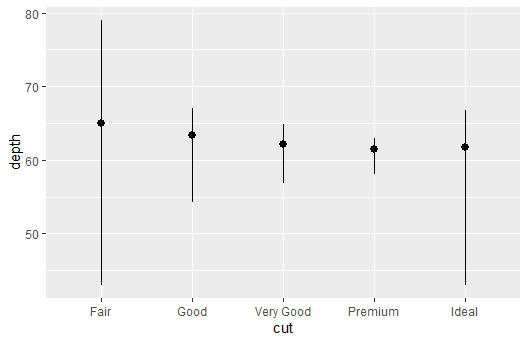
\includegraphics{Homework-4.sa_files/figure-latex/unnamed-chunk-2-1.pdf}

\begin{center}\rule{0.5\linewidth}{0.5pt}\end{center}

\hypertarget{exercise-2}{%
\subsubsection{(2) 23.2.1 Exercise 2}\label{exercise-2}}

One way to make linear models more robust is to use a different distance
measure. For example, instead of root-mean-squared (RMS) distance, you
could use mean-absolute-deviation (MAD) distance:

Use \texttt{optim()} to fit this model to the simulated data above and
visually compare it to the linear model, again examining at least 6
instances. You want both models to be drawn on top of each instance of
the simulated data set. Discuss what you find.

\emph{Hints}: \texttt{make\_prediction()} is not a built-in function;
you will need to create your own linear function. Unlike Exercise 1,
here you should only compare the models graphically; I don't think the
\(R^2\) metric is meaningful for a model that uses the MAD distance
measure.

\begin{Shaded}
\begin{Highlighting}[]
\CommentTok{\# I understand the code below is not very optimized but I could not figure out how to make a proper looping function because I kept getting the error "data$y is closure variable".}

\CommentTok{\# The two models perform very similarly on each iteration; however the RMS model is more effected by outlier data than the MAD model is. }




\NormalTok{sum }\OtherTok{\textless{}{-}} \DecValTok{0}

\ControlFlowTok{repeat}\NormalTok{\{}
\NormalTok{ sum }\OtherTok{\textless{}{-}}\NormalTok{ sum }\SpecialCharTok{+} \DecValTok{1}
 
 \ControlFlowTok{if}\NormalTok{ (sum }\SpecialCharTok{==} \DecValTok{7}\NormalTok{)\{}
  \ControlFlowTok{break}
\NormalTok{ \}}


\NormalTok{model1 }\OtherTok{\textless{}{-}} \ControlFlowTok{function}\NormalTok{(a, data) \{}
\NormalTok{  a[}\DecValTok{1}\NormalTok{] }\SpecialCharTok{+}\NormalTok{ data}\SpecialCharTok{$}\NormalTok{x }\SpecialCharTok{*}\NormalTok{ a[}\DecValTok{2}\NormalTok{]}
\NormalTok{\}}

\NormalTok{measure\_distanceMAD }\OtherTok{\textless{}{-}} \ControlFlowTok{function}\NormalTok{(mod, data) \{}
\NormalTok{  diff }\OtherTok{\textless{}{-}}\NormalTok{ data}\SpecialCharTok{$}\NormalTok{y }\SpecialCharTok{{-}} \FunctionTok{model1}\NormalTok{(mod, data)}
  \FunctionTok{mean}\NormalTok{(}\FunctionTok{abs}\NormalTok{(diff))}
\NormalTok{\}}

\NormalTok{measure\_distanceRMS }\OtherTok{\textless{}{-}} \ControlFlowTok{function}\NormalTok{(mod, data) \{}
\NormalTok{  diff }\OtherTok{\textless{}{-}}\NormalTok{ data}\SpecialCharTok{$}\NormalTok{y }\SpecialCharTok{{-}} \FunctionTok{model1}\NormalTok{(mod, data)}
  \FunctionTok{sqrt}\NormalTok{(}\FunctionTok{mean}\NormalTok{(diff }\SpecialCharTok{\^{}} \DecValTok{2}\NormalTok{))}
\NormalTok{\}}

\NormalTok{sim1a }\OtherTok{\textless{}{-}} \FunctionTok{tibble}\NormalTok{(}
  \AttributeTok{x =} \FunctionTok{rep}\NormalTok{(}\DecValTok{1}\SpecialCharTok{:}\DecValTok{10}\NormalTok{, }\AttributeTok{each =} \DecValTok{3}\NormalTok{),}
  \AttributeTok{y =}\NormalTok{ x }\SpecialCharTok{*} \FloatTok{1.5} \SpecialCharTok{+} \DecValTok{6} \SpecialCharTok{+} \FunctionTok{rt}\NormalTok{(}\FunctionTok{length}\NormalTok{(x), }\AttributeTok{df =} \DecValTok{2}\NormalTok{)}
\NormalTok{)}

\NormalTok{best1 }\OtherTok{\textless{}{-}} \FunctionTok{optim}\NormalTok{(}\FunctionTok{c}\NormalTok{(}\DecValTok{0}\NormalTok{,}\DecValTok{0}\NormalTok{), measure\_distanceMAD, }\AttributeTok{data =}\NormalTok{ sim1a)}
\NormalTok{best2 }\OtherTok{\textless{}{-}} \FunctionTok{optim}\NormalTok{(}\FunctionTok{c}\NormalTok{(}\DecValTok{0}\NormalTok{,}\DecValTok{0}\NormalTok{), measure\_distanceRMS, }\AttributeTok{data =}\NormalTok{ sim1a)}

\NormalTok{plot1 }\OtherTok{\textless{}{-}} \FunctionTok{ggplot}\NormalTok{(sim1a, }\FunctionTok{aes}\NormalTok{(x, y)) }\SpecialCharTok{+} 
  \FunctionTok{geom\_point}\NormalTok{() }\SpecialCharTok{+} 
  \FunctionTok{geom\_abline}\NormalTok{(}\AttributeTok{intercept =}\NormalTok{ best1}\SpecialCharTok{$}\NormalTok{par[}\DecValTok{1}\NormalTok{], }\AttributeTok{slope =}\NormalTok{ best1}\SpecialCharTok{$}\NormalTok{par[}\DecValTok{2}\NormalTok{], }\AttributeTok{color =} \StringTok{"red"}\NormalTok{)}\SpecialCharTok{+}
  \FunctionTok{geom\_abline}\NormalTok{(}\AttributeTok{intercept =}\NormalTok{ best2}\SpecialCharTok{$}\NormalTok{par[}\DecValTok{1}\NormalTok{],}\AttributeTok{slope =}\NormalTok{ best2}\SpecialCharTok{$}\NormalTok{par[}\DecValTok{2}\NormalTok{], }\AttributeTok{color =} \StringTok{"blue"}\NormalTok{)}

\FunctionTok{print}\NormalTok{(plot1)}

\NormalTok{\}}
\end{Highlighting}
\end{Shaded}

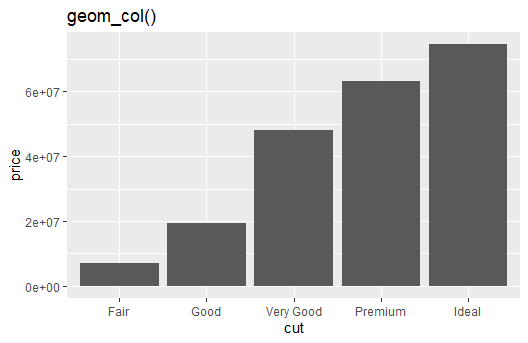
\includegraphics{Homework-4.sa_files/figure-latex/unnamed-chunk-3-1.pdf}
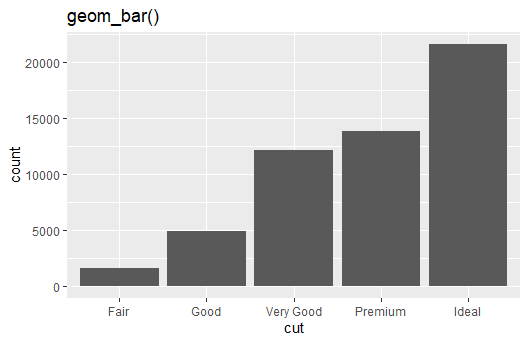
\includegraphics{Homework-4.sa_files/figure-latex/unnamed-chunk-3-2.pdf}
\includegraphics{Homework-4.sa_files/figure-latex/unnamed-chunk-3-3.pdf}
\includegraphics{Homework-4.sa_files/figure-latex/unnamed-chunk-3-4.pdf}
\includegraphics{Homework-4.sa_files/figure-latex/unnamed-chunk-3-5.pdf}
\includegraphics{Homework-4.sa_files/figure-latex/unnamed-chunk-3-6.pdf}

\begin{center}\rule{0.5\linewidth}{0.5pt}\end{center}

\hypertarget{exercises-1}{%
\subsection{23.3.3 Exercises}\label{exercises-1}}

\hypertarget{exercise-1-1}{%
\subsubsection{(3) 23.3.3 Exercise 1}\label{exercise-1-1}}

Instead of using \texttt{lm()} to fit a straight line, you can use
\texttt{loess()} to fit a smooth curve. Repeat the process of model
fitting, grid generation, predictions, and visualization on
\texttt{sim1} using \texttt{loess()} instead of \texttt{lm()}. How does
the result compare to \texttt{geom\_smooth()}?

\begin{Shaded}
\begin{Highlighting}[]
\CommentTok{\# \textquotesingle{}geom\_smooth()\textquotesingle{} uses \textquotesingle{}loess()\textquotesingle{} as a default so they should look exactly the same. }

\NormalTok{sim1\_loess }\OtherTok{\textless{}{-}} \FunctionTok{loess}\NormalTok{(y }\SpecialCharTok{\textasciitilde{}}\NormalTok{ x, }\AttributeTok{data =}\NormalTok{ sim1)}

\NormalTok{grid\_loess }\OtherTok{\textless{}{-}}\NormalTok{ sim1 }\SpecialCharTok{\%\textgreater{}\%}
  \FunctionTok{add\_predictions}\NormalTok{(sim1\_loess)}

\NormalTok{sim1 }\OtherTok{\textless{}{-}}\NormalTok{ sim1 }\SpecialCharTok{\%\textgreater{}\%}
  \FunctionTok{add\_residuals}\NormalTok{(sim1\_loess, }\AttributeTok{var =} \StringTok{"resid\_loess"}\NormalTok{) }\SpecialCharTok{\%\textgreater{}\%}
  \FunctionTok{add\_predictions}\NormalTok{(sim1\_loess, }\AttributeTok{var =} \StringTok{"pred\_loess"}\NormalTok{)}

\NormalTok{plot\_sim1\_loess }\OtherTok{\textless{}{-}}
  \FunctionTok{ggplot}\NormalTok{(sim1, }\FunctionTok{aes}\NormalTok{(}\AttributeTok{x =}\NormalTok{ x, }\AttributeTok{y =}\NormalTok{ y)) }\SpecialCharTok{+}
  \FunctionTok{geom\_line}\NormalTok{(}\FunctionTok{aes}\NormalTok{(}\AttributeTok{x =}\NormalTok{ x, }\AttributeTok{y =}\NormalTok{ pred), }\AttributeTok{data =}\NormalTok{ grid\_loess, }\AttributeTok{colour =} \StringTok{"blue"}\NormalTok{)}\SpecialCharTok{+}
  \FunctionTok{geom\_smooth}\NormalTok{(}\AttributeTok{colour =} \StringTok{"red"}\NormalTok{, }\AttributeTok{se =} \ConstantTok{FALSE}\NormalTok{)}
\NormalTok{plot\_sim1\_loess}
\end{Highlighting}
\end{Shaded}

\begin{verbatim}
## `geom_smooth()` using method = 'loess' and formula 'y ~ x'
\end{verbatim}

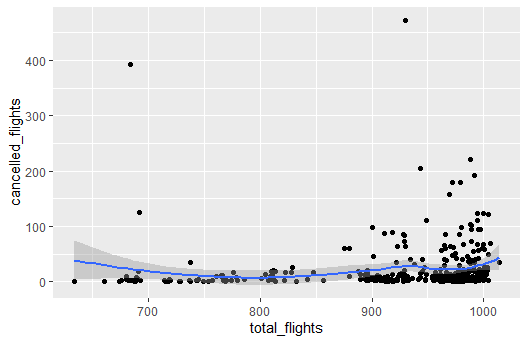
\includegraphics{Homework-4.sa_files/figure-latex/unnamed-chunk-4-1.pdf}

\hypertarget{exercise-2-1}{%
\subsubsection{(4) 23.3.3 Exercise 2}\label{exercise-2-1}}

\texttt{add\_predictions()} is paired with
\texttt{gather\_predictions()} and \texttt{spread\_predictions()}. Use
both \texttt{gather\_predictions()} and \texttt{spread\_predictions()}
to repeat the analysis with the two models used in problem (3) above.
How do these three functions differ?

\begin{Shaded}
\begin{Highlighting}[]
\CommentTok{\# The functions differ on how the data is stored. The gather predictions first selects one model then runs predictions on each model separately. Spread instead uses the same x and shows the result of each machine learning technique side by side. Personally, I see spread being the more useful and more effective calling of the predictions.}


\CommentTok{\# Assumed the second model is supposed to be \textquotesingle{}lm()\textquotesingle{}}

\NormalTok{sim1\_mod }\OtherTok{\textless{}{-}} \FunctionTok{lm}\NormalTok{(y }\SpecialCharTok{\textasciitilde{}}\NormalTok{ x, }\AttributeTok{data =}\NormalTok{ sim1)}
\NormalTok{grid }\OtherTok{\textless{}{-}}\NormalTok{ sim1 }\SpecialCharTok{\%\textgreater{}\%}
  \FunctionTok{data\_grid}\NormalTok{(x)}

\NormalTok{grid }\SpecialCharTok{\%\textgreater{}\%}
  \FunctionTok{gather\_predictions}\NormalTok{(sim1\_mod, sim1\_loess)}
\end{Highlighting}
\end{Shaded}

\begin{verbatim}
## # A tibble: 20 x 3
##    model          x  pred
##    <chr>      <int> <dbl>
##  1 sim1_mod       1  6.27
##  2 sim1_mod       2  8.32
##  3 sim1_mod       3 10.4 
##  4 sim1_mod       4 12.4 
##  5 sim1_mod       5 14.5 
##  6 sim1_mod       6 16.5 
##  7 sim1_mod       7 18.6 
##  8 sim1_mod       8 20.6 
##  9 sim1_mod       9 22.7 
## 10 sim1_mod      10 24.7 
## 11 sim1_loess     1  5.34
## 12 sim1_loess     2  8.27
## 13 sim1_loess     3 10.8 
## 14 sim1_loess     4 12.8 
## 15 sim1_loess     5 14.6 
## 16 sim1_loess     6 16.6 
## 17 sim1_loess     7 18.7 
## 18 sim1_loess     8 20.8 
## 19 sim1_loess     9 22.6 
## 20 sim1_loess    10 24.0
\end{verbatim}

\begin{Shaded}
\begin{Highlighting}[]
\NormalTok{grid }\SpecialCharTok{\%\textgreater{}\%}
  \FunctionTok{spread\_predictions}\NormalTok{(sim1\_mod, sim1\_loess)}
\end{Highlighting}
\end{Shaded}

\begin{verbatim}
## # A tibble: 10 x 3
##        x sim1_mod sim1_loess
##    <int>    <dbl>      <dbl>
##  1     1     6.27       5.34
##  2     2     8.32       8.27
##  3     3    10.4       10.8 
##  4     4    12.4       12.8 
##  5     5    14.5       14.6 
##  6     6    16.5       16.6 
##  7     7    18.6       18.7 
##  8     8    20.6       20.8 
##  9     9    22.7       22.6 
## 10    10    24.7       24.0
\end{verbatim}

\hypertarget{exercise-3}{%
\subsubsection{(5) 23.3.3 Exercise 3}\label{exercise-3}}

What does \texttt{geom\_ref\_line()} do? What package does it come from?
Why is displaying a reference line in plots showing residuals useful and
important?

\begin{Shaded}
\begin{Highlighting}[]
\CommentTok{\# It simply adds a reference line through all the graphs to easier see the correlation.}

\NormalTok{mod1 }\OtherTok{\textless{}{-}} \FunctionTok{lm}\NormalTok{(y }\SpecialCharTok{\textasciitilde{}}\NormalTok{ x1 }\SpecialCharTok{+}\NormalTok{ x2, }\AttributeTok{data =}\NormalTok{ sim3)}
\NormalTok{mod2 }\OtherTok{\textless{}{-}} \FunctionTok{lm}\NormalTok{(y }\SpecialCharTok{\textasciitilde{}}\NormalTok{ x1 }\SpecialCharTok{*}\NormalTok{ x2, }\AttributeTok{data =}\NormalTok{ sim3)}

\NormalTok{grid }\OtherTok{\textless{}{-}}\NormalTok{ sim3 }\SpecialCharTok{\%\textgreater{}\%}
  \FunctionTok{data\_grid}\NormalTok{(x1, x2) }\SpecialCharTok{\%\textgreater{}\%}
  \FunctionTok{gather\_predictions}\NormalTok{(mod1, mod2)}
\NormalTok{grid}
\end{Highlighting}
\end{Shaded}

\begin{verbatim}
## # A tibble: 80 x 4
##    model    x1 x2     pred
##    <chr> <int> <fct> <dbl>
##  1 mod1      1 a      1.67
##  2 mod1      1 b      4.56
##  3 mod1      1 c      6.48
##  4 mod1      1 d      4.03
##  5 mod1      2 a      1.48
##  6 mod1      2 b      4.37
##  7 mod1      2 c      6.28
##  8 mod1      2 d      3.84
##  9 mod1      3 a      1.28
## 10 mod1      3 b      4.17
## # ... with 70 more rows
\end{verbatim}

\begin{Shaded}
\begin{Highlighting}[]
\NormalTok{sim3r }\OtherTok{\textless{}{-}}\NormalTok{ sim3 }\SpecialCharTok{\%\textgreater{}\%}
  \FunctionTok{gather\_residuals}\NormalTok{(mod1, mod2)}
\NormalTok{sim3r}
\end{Highlighting}
\end{Shaded}

\begin{verbatim}
## # A tibble: 240 x 7
##    model    x1 x2      rep      y    sd   resid
##    <chr> <int> <fct> <int>  <dbl> <dbl>   <dbl>
##  1 mod1      1 a         1 -0.571     2 -2.25  
##  2 mod1      1 a         2  1.18      2 -0.491 
##  3 mod1      1 a         3  2.24      2  0.562 
##  4 mod1      1 b         1  7.44      2  2.87  
##  5 mod1      1 b         2  8.52      2  3.96  
##  6 mod1      1 b         3  7.72      2  3.16  
##  7 mod1      1 c         1  6.51      2  0.0261
##  8 mod1      1 c         2  5.79      2 -0.691 
##  9 mod1      1 c         3  6.07      2 -0.408 
## 10 mod1      1 d         1  2.11      2 -1.92  
## # ... with 230 more rows
\end{verbatim}

\begin{Shaded}
\begin{Highlighting}[]
\FunctionTok{ggplot}\NormalTok{(sim3r, }\FunctionTok{aes}\NormalTok{(}\AttributeTok{x =}\NormalTok{ x1, }\AttributeTok{y =}\NormalTok{ resid, }\AttributeTok{color =}\NormalTok{ x2)) }\SpecialCharTok{+}
  \FunctionTok{geom\_ref\_line}\NormalTok{(}\AttributeTok{h =} \DecValTok{0}\NormalTok{, }\AttributeTok{colour =} \StringTok{\textquotesingle{}red\textquotesingle{}}\NormalTok{) }\SpecialCharTok{+}
  \FunctionTok{geom\_point}\NormalTok{() }\SpecialCharTok{+}
  \FunctionTok{facet\_grid}\NormalTok{(}\AttributeTok{rows =} \FunctionTok{vars}\NormalTok{(model), }\AttributeTok{cols =} \FunctionTok{vars}\NormalTok{(x2))}
\end{Highlighting}
\end{Shaded}

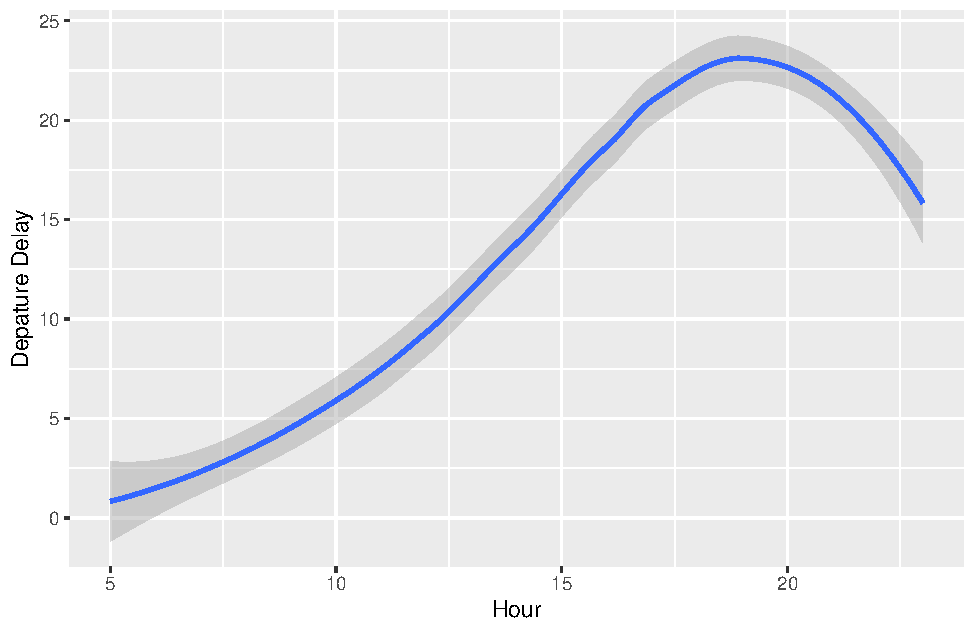
\includegraphics{Homework-4.sa_files/figure-latex/unnamed-chunk-6-1.pdf}

\hypertarget{exercise-4}{%
\subsubsection{(6) 23.3.3 Exercise 4}\label{exercise-4}}

Why might you want to look at a frequency polygon of absolute residuals?
What are the pros and cons compared to looking at the raw residuals?

\begin{Shaded}
\begin{Highlighting}[]
\CommentTok{\# Since the direction of the residual does not matter, it allows the user to more effectively see the the values of the residual.}


\NormalTok{sim1 }\OtherTok{\textless{}{-}}\NormalTok{ sim1 }\SpecialCharTok{\%\textgreater{}\%}
  \FunctionTok{add\_residuals}\NormalTok{(sim1\_mod)}

\FunctionTok{ggplot}\NormalTok{(sim1, }\FunctionTok{aes}\NormalTok{(}\AttributeTok{x =} \FunctionTok{abs}\NormalTok{(resid))) }\SpecialCharTok{+}
  \FunctionTok{geom\_freqpoly}\NormalTok{(}\AttributeTok{binwidth =} \FloatTok{0.5}\NormalTok{)}
\end{Highlighting}
\end{Shaded}

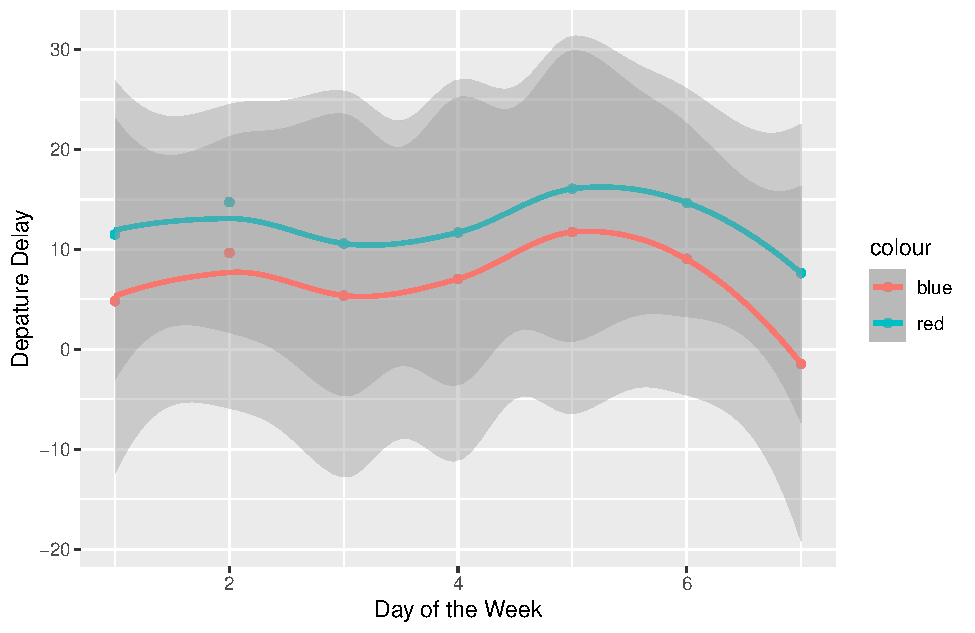
\includegraphics{Homework-4.sa_files/figure-latex/unnamed-chunk-7-1.pdf}

\begin{Shaded}
\begin{Highlighting}[]
\FunctionTok{ggplot}\NormalTok{(sim1, }\FunctionTok{aes}\NormalTok{(}\AttributeTok{x =}\NormalTok{ resid)) }\SpecialCharTok{+}
  \FunctionTok{geom\_freqpoly}\NormalTok{(}\AttributeTok{binwidth =} \FloatTok{0.5}\NormalTok{)}
\end{Highlighting}
\end{Shaded}

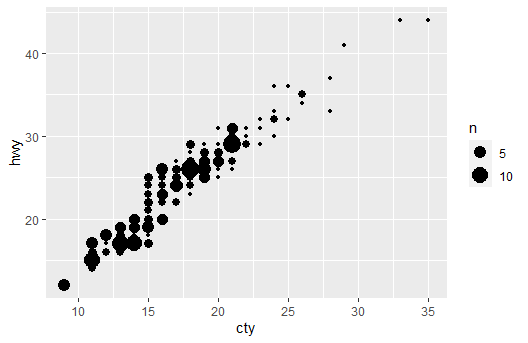
\includegraphics{Homework-4.sa_files/figure-latex/unnamed-chunk-7-2.pdf}

\begin{center}\rule{0.5\linewidth}{0.5pt}\end{center}

\hypertarget{exercises-2}{%
\subsection{23.4.5 Exercises}\label{exercises-2}}

\hypertarget{exercise-4-1}{%
\subsubsection{(7) 23.4.5 Exercise 4}\label{exercise-4-1}}

For \texttt{sim4}, which of \texttt{mod1} and \texttt{mod2} is better?
The book author believes that \texttt{mod2} does a slightly better job
at removing patterns, but claims the effects are subtle. Examine the
\(R^2\) values for the two models, and develop a plot that attempts to
support this claim. In the end, how well does your plot support the
claim? How likely is it that the claim is true?

\begin{Shaded}
\begin{Highlighting}[]
\CommentTok{\# I mean the R\^{}2 score shows that both models are not particularly good at predicting, the mod2 has a better score but when it is that close to .50 then both models are just not good enough to be used. In the plot, it can be seen that the mod2 has a more condense residual spread, but still not enough to be viable.}
\end{Highlighting}
\end{Shaded}

\begin{Shaded}
\begin{Highlighting}[]
\NormalTok{mod1 }\OtherTok{\textless{}{-}} \FunctionTok{lm}\NormalTok{(y }\SpecialCharTok{\textasciitilde{}}\NormalTok{ x1 }\SpecialCharTok{+}\NormalTok{ x2, }\AttributeTok{data =}\NormalTok{ sim4)}
\NormalTok{mod2 }\OtherTok{\textless{}{-}} \FunctionTok{lm}\NormalTok{(y }\SpecialCharTok{\textasciitilde{}}\NormalTok{ x1 }\SpecialCharTok{*}\NormalTok{ x2, }\AttributeTok{data =}\NormalTok{ sim4)}
\end{Highlighting}
\end{Shaded}

\begin{Shaded}
\begin{Highlighting}[]
\NormalTok{grid }\OtherTok{\textless{}{-}}\NormalTok{ sim4 }\SpecialCharTok{\%\textgreater{}\%}
  \FunctionTok{data\_grid}\NormalTok{(x1,x2)}
\NormalTok{grid }\OtherTok{\textless{}{-}}\NormalTok{ grid }\SpecialCharTok{\%\textgreater{}\%}
  \FunctionTok{gather\_predictions}\NormalTok{(mod1, mod2)}

\NormalTok{sim4\_mods }\OtherTok{\textless{}{-}} \FunctionTok{gather\_residuals}\NormalTok{(sim4, mod1, mod2)}
\end{Highlighting}
\end{Shaded}

\begin{Shaded}
\begin{Highlighting}[]
\NormalTok{m1r }\OtherTok{\textless{}{-}} \FunctionTok{summary}\NormalTok{(mod1)}\SpecialCharTok{$}\NormalTok{r.squared}
\NormalTok{m2r }\OtherTok{\textless{}{-}} \FunctionTok{summary}\NormalTok{(mod2)}\SpecialCharTok{$}\NormalTok{r.squared}
\FunctionTok{print}\NormalTok{(}\FunctionTok{sprintf}\NormalTok{(}\StringTok{"mod1 R\^{}2: \%.1f\%\%"}\NormalTok{, m1r}\SpecialCharTok{*}\DecValTok{100}\NormalTok{))}
\end{Highlighting}
\end{Shaded}

\begin{verbatim}
## [1] "mod1 R^2: 50.5%"
\end{verbatim}

\begin{Shaded}
\begin{Highlighting}[]
\FunctionTok{print}\NormalTok{(}\FunctionTok{sprintf}\NormalTok{(}\StringTok{"mod2 R\^{}2: \%.1f\%\%"}\NormalTok{, m2r}\SpecialCharTok{*}\DecValTok{100}\NormalTok{))}
\end{Highlighting}
\end{Shaded}

\begin{verbatim}
## [1] "mod2 R^2: 52.2%"
\end{verbatim}

\begin{Shaded}
\begin{Highlighting}[]
\FunctionTok{print}\NormalTok{(}\FunctionTok{sprintf}\NormalTok{(}\StringTok{"R\^{}2\_mod2 {-} R\^{}2\_mod1: \%.1f\%\%"}\NormalTok{, (m2r }\SpecialCharTok{{-}}\NormalTok{ m1r)}\SpecialCharTok{*}\DecValTok{100}\NormalTok{))}
\end{Highlighting}
\end{Shaded}

\begin{verbatim}
## [1] "R^2_mod2 - R^2_mod1: 1.7%"
\end{verbatim}

\begin{Shaded}
\begin{Highlighting}[]
\FunctionTok{ggplot}\NormalTok{(sim4\_mods, }\FunctionTok{aes}\NormalTok{(}\AttributeTok{x =}\NormalTok{ x1, }\AttributeTok{y =}\NormalTok{ resid, }\AttributeTok{color =}\NormalTok{ x2)) }\SpecialCharTok{+}
  \FunctionTok{geom\_ref\_line}\NormalTok{(}\AttributeTok{h =} \DecValTok{0}\NormalTok{, }\AttributeTok{colour =} \StringTok{\textquotesingle{}red\textquotesingle{}}\NormalTok{) }\SpecialCharTok{+}
  \FunctionTok{geom\_point}\NormalTok{() }\SpecialCharTok{+}
  \FunctionTok{facet\_grid}\NormalTok{(}\AttributeTok{rows =} \FunctionTok{vars}\NormalTok{(model), }\AttributeTok{cols =} \FunctionTok{vars}\NormalTok{(x2))}
\end{Highlighting}
\end{Shaded}

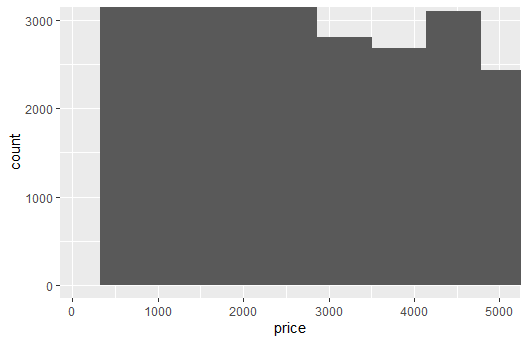
\includegraphics{Homework-4.sa_files/figure-latex/unnamed-chunk-12-1.pdf}

\end{document}
